\chapter{CESM surface concentration correction model}
\label{sec:appA}
\raggedbottom

\clearpage


\section{Introduction}

Due to computational storage capacity limitations certain variables were only saved as monthly averages. Supplementary Material S1 details the diagnostic model used to approximate surface phytoplankton carbon concentrations for calculations at daily
resolution

\section{CESM surface concentration correction factor}

Due to computational storage capacity limitations surface phytoplankton carbon
concentrations were only saved at the monthly resolution and thus must be approximated
for calculations at daily resolution.

Our first approximation assumes a homogeneously distributed vertical profile in
which all biomass is stored evenly within the greater of the mixed layer or euphotic depth (referred to as the $Profile Depth, Z_{profile} = max(MLD, Z_{eu})$). Under this assumption the surface concentration (also equivalent to the mean concentration) is calculated by dividing the vertical inventory ($\Sigma C_{phyto}$) by $Z_{profile}$ (see \textbf{Sec. 2.3.3}).

This assumption holds well for deep, well mixed, mixed layers that exceed the
euphotic depth \parencite{BossObservationspigmentparticle2008,Bosssituevaluationinitiation2010, BehrenfeldAnnualcyclesecological2013}.However the surface concentrations of shallower profiles, where phytoplankton growth can persist in stratified water below the mixed layer, are not approximated as well. In order to improve our approximations, we weight the surface concentration of shallow profiles ($Z_{profile} <100m$) by a spatially and depth dependent correction factor.

\section{Correction factor model}

We use explicitly resolved monthly surface concentrations to create a model to
approximate the true correction factor as a function of grid cell and $Z_{profile}$.

To do so, we first approximate the monthly surface concentration using the first
order approximation defined above and $\Sigma C_{phyto}$ and $Z_{profile}$ values calculated as described in \textbf{Sec. 2.3.3} but from monthly means,

\begin{equation}
    [C_{phyto}]_{surf \; approx} = \frac{\Sigma C_{phyto} }{Z_{profile}}.
\end{equation}

\noindent{We then divide the true surface concentration by the approximated to calculate the correction factor, $Cor_{factor}$}


\begin{equation}
    Cor_{factor} = \frac{[C_{phyto}]_{surf \; true}}{[C_{phyto}]_{surf \; approx}} .
\end{equation}

Distributions of $Cor_{factor}$ as a function of $Z_{profile}$ at each model grid point are then fit to a simple model, such that we can model the requisite $Cor_{factor}$ of the daily data given a grid cell and $Z_{profile}$.

\textbf{Figure A2.1.1} shows a typical distribution in which $Cor_{factor}$ approaches 1.0 as the $Z_{profile}$ reaches 100m (See \textbf{Figure A2.1.1}). Our simple model fits a linear regression to all points where $Z_{profile} \< 100m$ and assigns a $Cor_{factor}$ of 1.0 where $Z_{profile} \>100m$ where our uniform distribution assumption is acceptable.

An independent function is modeled at each grid point and compiled. With this
model, we can now assign a reasonably well-estimated $Cor_{factor}$ for any particular
spatial coordinate and $Z_{profile}$ at the daily resolution.


%%%%%%%%%%%%%%%%%%%%%%%%%%%
\section{Test of model skill}

We use monthly mean values of $\Sigma C_{phyto}$ and $Z_{profile}$  and our correction factor model to compute corrected approximate surface concentrations that can be directly
compared to the true surface concentrations stored at the monthly resolution to test model skill.

In \textbf{Fig. A2.1.2}, plotting time series from one year at the same grid point modeled in \textbf{Fig. A2.1.1}, it is clear the corrected values match the true values much better than our initial approximation (\textbf{Eq}. A2.1.1).

We test the skill of the approximated values at each grid cell. \textbf{Fig. A2.1.3a} projects the mean absolute value percent deviation of the corrected approximation from the true surface values. Error ranges from 5-15\%. More importantly, figure \textbf{Fig. A2.1.3b} shows consistently high ($r\>.95$) correlations between the two time series across the Southern Ocean. Thus despite minor discrepancies in the absolute magnitude, seasonal trends (our primary concern) remain tightly coupled. \textbf{Table A2.1} outlines the percent deviation and correlation coefficient values spatially averaged over each swath considered in \textbf{Sec. 2.4.2 and 2.4.3} in addition to the entire Southern Hemisphere.


%%%%%%%%%%%%%%%%%%%%%%%%%%%%%%%%%%%%%%%%%%
        %%     Figures  %%
%%%%%%%%%%%%%%%%%%%%%%%%%%%%%%%%%%%%%%%%%%



%%%%%%%%%%%%%%%%%%%%%%%%
%%%%%% Figure 1 %%%%%%%%
%%%%%%%%%%%%%%%%%%%%%%%%


\begin{figure}[!htbp]
\begin{adjustwidth}{-1in}{-1in}
 \centering
 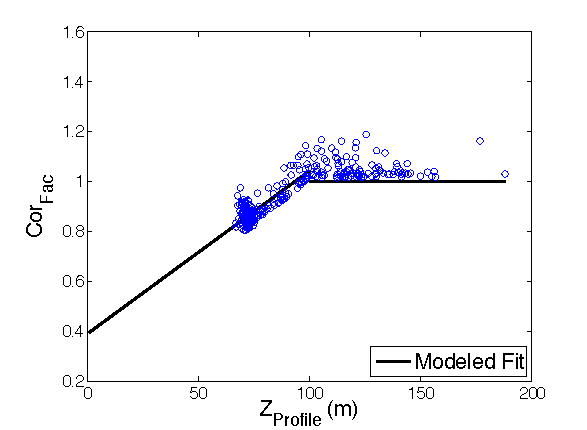
\includegraphics[scale=1.5]{figures/A1/Figure1.pdf}
\end{adjustwidth}
\caption[$Cor_{Factor}$ model fit]{The $Cor_{Factor}$ needed to convert the approximated surface concentration to the true surface
concentration plotted as a function of $Z_{profile}$ for the timeseries at a single grid point (Lat = 50$^\circ$ S, Lon = 91$^\circ$ W)
and monthly resolution. The modeled fit is plotted in black.}
\label{fig:Fig1}
\end{figure}



%%%%%%%%%%%%%%%%%%%%%%%%
%%%%%% Figure 2 %%%%%%%%
%%%%%%%%%%%%%%%%%%%%%%%%


\begin{figure}[!htbp]
\begin{adjustwidth}{-1in}{-1in}
 \centering
 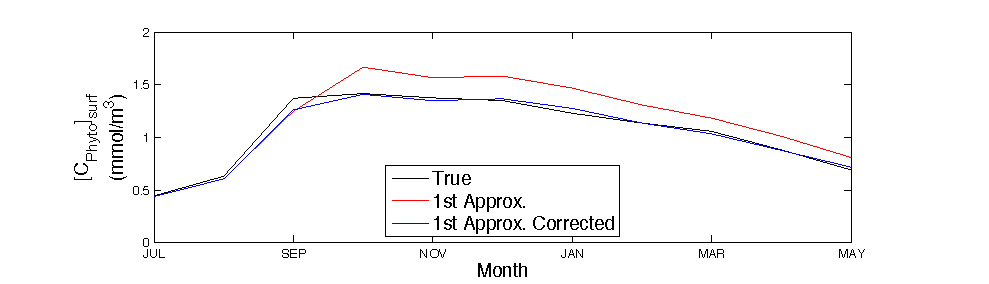
\includegraphics[scale=1.3]{figures/A1/Figure2.pdf}
\end{adjustwidth}
\caption[Time Series of {$[C_{phyto}]_{surf}$}]{A single year, monthly resolution time series plotted for the true surface phytoplankton biomass
concentration (black trace) along a first approximation (red trace) and the corrected approximation (blue trace). Time series are from the same grid cell as Fig. A1 (Lat = 50$^\circ$ S, Lon =91$^\circ$ W ).  }
\label{fig:Fig2}
\end{figure}


%%%%%%%%%%%%%%%%%%%%%%%%
%%%%%% Figure 3 %%%%%%%%
%%%%%%%%%%%%%%%%%%%%%%%%


\begin{figure}[!htbp]
\begin{adjustwidth}{-1in}{-1in}
 \centering
 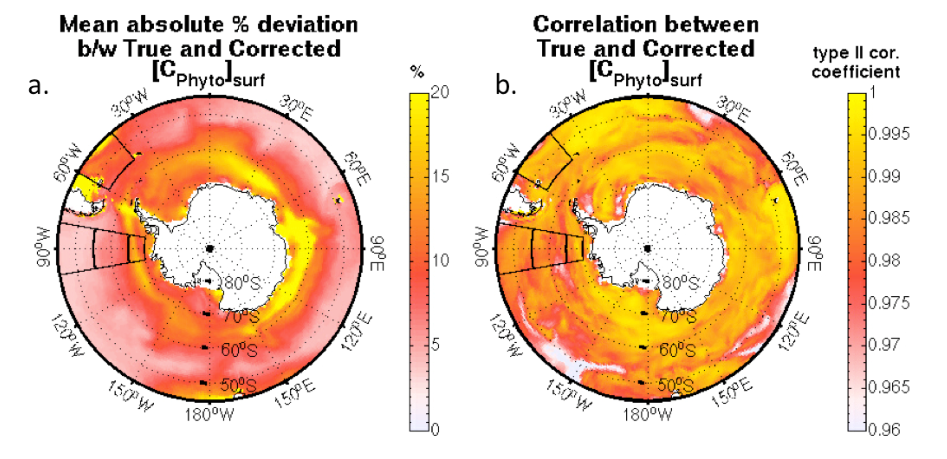
\includegraphics[scale=1.2]{figures/A1/Figure3.pdf}
\end{adjustwidth}
\caption[Model Skill]{The mean absolute value percent deviation of the corrected approximation from the true surface
values for each grid cell is plotted on the left (\textbf{a}) with correlation coefficient between the two time series plotted on the right (\textbf{b}). }
\label{fig:Fig3}
\end{figure}


%%%%%%%%%%%%%%%%%%%%%%%%%%%%%%%%%%%%%%%%%%
        %%     Tables  %%
%%%%%%%%%%%%%%%%%%%%%%%%%%%%%%%%%%%%%%%%%%

\begin{table}[!htbp]
 \begin{center}
 \begin{tabular}{ |c|c|c|c|c|c| } 
  \hline
   & P1 & P2 & P3 & A1 & SH \\ 
  \hline
   Mean \% Deviation & 3.83 & 6.53 & 11.75 & 12.04 & 10.98 \\ 
  \hline
   Correlation Coefficient & .984 & .983 & .987 &  .988 & .82 \\ 
  \hline
 \end{tabular}
 \end{center}
 \caption[Model Skill]{The percent deviation and correlation coefficient values spatially averaged over each swath
considered in \textbf{Sec. 2.4.2} and \textbf{2.4.3} in addition to the entire Southern Hemisphere (SH).}

\end{table}